
\section{Ejercicio 2: Menos es más}
    % 1. Describir detalladamente el problema a resolver dando ejemplos del mismo y sus soluciones.

	\begin{figure}[ht]
		\begin{center}
			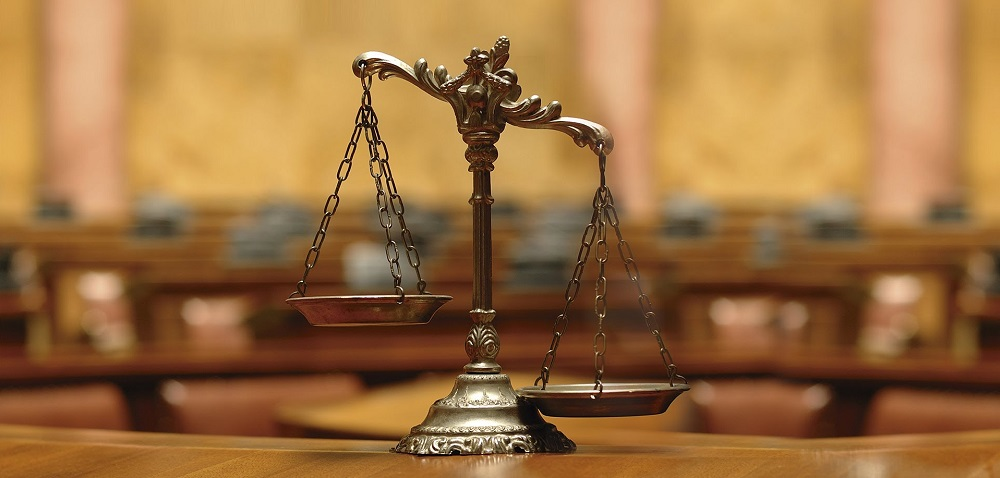
\includegraphics[width=0.5\columnwidth]{imagenes/balanza.jpg}
			\caption{Equilibro}
		\end{center}
	\end{figure}

	\subsection{Descripción del problema}
	En su destino hacia la cruz en el mapa recorrieron varias salas distintas. Se dieron cuenta que en cada sala se iban encontrando con un fragmento de una tabla con un mansucrito antiguo. Por lo tanto, antes de continuar, quieren juntarlos todos.\par
	A medida que se iban abriendo camino se dieron cuenta que ciertas paredes derribables requerían cierto esfuerzo para
	abrirse. Este esfuerzo será representado por un $n\in{\mathbb{n}}$ donde $n < 10$. Luego, teniendo un mapa de $F*C$ (F = Filas y C = Columnas), donde se indique el $n$ en las paredes derribables, quieren encontrar cual es el mı́nimo esfuerzo que deben hacer para acceder a todas las salas. \par

	Por lo tanto, se deberá pasar por parametro al algoritmo, el mapa con sus paredes y el esfuerzo para romperlas. 
	\newline
	~

	\textbf{Formato de entrada:} La primer lı́nea consta de dos enteros positivos F y C, donde F es la cantidad de filas en el mapa, y C es la cantidad de columnas. Las siguientes F filas contienen C caracteres. Un “.” representa un lugar caminable, los números del 1 al 9 indican el esfuerzo en romper esa pared, un “\#” representa una pared indestructible. Las paredes con más de 2 paredes adyacentes son indestructibles (contendran un “\#”). Las paredes con menos de 2 paredes adyacentes son indestructibles (contendran un “\#”). Dos salas se pueden conectar si existe una pared adyacente a las dos salas que se puede destruir (Es decir, no quedan conectadas si se rompen muchas parede adyacentes). Por último, los bordes del mapa tendrán un “\#”.


	\begin{verbatim}
    F C
    F_1
    ...
    F_n
    \end{verbatim}
    

	~

	\textbf{Salida:} La salida consta de un número indicando el esfuerzo que debe hacer el equipo para acceder a todas las salas. Si no es posible recorrer todas las salas se imprime un −1. La salida tendrá el siguiente formato:\par
	
	\begin{tabular}{ll}
		\texttt{E}
	\end{tabular}


	%DOY UN EJEMPLO

	~

	Se tiene como restricción que $F$ y $C$ está en el siguiente rango: 1$<=$ $F,C$ $<=$ $10^{4}$. La complejidad temporal debe ser a lo sumo $\ord(FC * \log{FC}{})$.

    % 2. Explicar de forma clara, sencilla, estructurada y concisa, las ideas desarrolladas para la resolución del problema. Utilizar pseudocódigo y lenguaje coloquial (no código fuente). Justificar por qué el procedimiento resuelve efectivamente el problema.
    
    \subsection{Solución propuesta}

    \subsubsection{Modelado}

    Para resolver este problema, se pedía encontrar el mínimo esfuerzo, para pasar por todas las salas del mapa. Para esto se usó el algoritmo de Kruskal, cuyo fín es encontrar el \textbf{Arbol Generador Mínimo} dentro de un grafo, cuyo pesos en las aristas sea positivo. En nuestro caso, esto representaría el mínimo esfuerzo, para poder visitar todas las salas. Para poder usar Kruskal, modelamos el problema en grafos. Para esto, se creó una matriz de $F*C$, donde fueron guardados los caractéres del mapa pasados como parámetro de entrada.\par
    Luego se usó esta matríz para generara los nodos y las aristas. Para esto, en principio cada posicion de la matriz es un nodo, numerados según la posición dentro de la matriz ($filaDelNodoActual * cantColumnas + columnaDelNodoActual$). \par
    Una vez generada la matríz, se la vuelve a recorrer, para generar las aristas. Sea nodoActual, el caracter ubicado en la posición de la matríz en la cual estoy queriendo generar una arista,

    \begin{itemize}
    	\item Si nodoActual es “\#”, no hago nada.
    	\item Caso contrario, me fijo si nodoActual es “.” o un número.
    	\begin{itemize}
    			\item Si es un “.”. Se debe fijar en la columna siguiente de la matriz, a este nodo lo llamaremos, nodoVecino.\par
 		   		Si nodoVecino es distinto de “\#”. Genero una arista, cuyo comienzo es el número de nodoActual, su fin es el de nodoVecino, y el peso es 0. Análogo para la posición inmediata dentro de la matriz, de la fila siguiente.
  		  		\item Si es un número. Deberá hacer lo mismo que en el caso anterior. Con la diferencia que, si uno de sus vecinos es también un número, no deberá hacer nada y que solo tendrá un vecino “.”, en la columna inmediata superior o, en la fila siguiente, dentro de la matriz, y cuyo peso de la arista, será el número del nodo.
 			   	\end{itemize}
    \end{itemize} 


    Luego para el siguiente mapa,

       	\begin{figure}[H]
		\begin{center}
			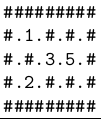
\includegraphics{imagenes/altoMapa.png}
			\caption{Mapa a modelar}
		\end{center}
	\end{figure}


    Queda el siguiente grafo,
    
   	\begin{figure}[H]
		\begin{center}
			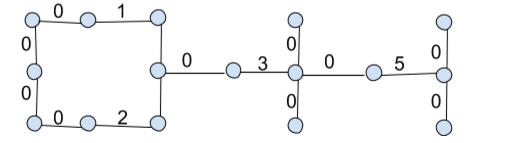
\includegraphics[scale=0.5]{imagenes/grafoOK.png}
			\caption{Grafo del mapa}
		\end{center}
	\end{figure}


    Cada una de estas aristas, es guardada en un vector de aristas.
    Luego, este vector de aristas, es usados como parámetro de entrada, en el algoritmo de Kruskal, quien devolverá la suma del \textbf{Arbol Generador Mínimo}. En caso de no tener solución, es decir, no poder recorrer el mapa, devolverá -1.



	\subsubsection{Implementación}\label{ej2_imp}


	Habiendo introducido la idea, se detalla el comportamiento del algoritmo para
	una entrada arbitraria. \par 

	La primera parte consiste en la inicialización de valores para el algoritmo. Se guardar la cantidad de filas y de columnas del mapa pasado por standard input. Se crea una matriz con este mismo tamaño. Luego se guardan en esta matriz, los caractéres pasados como parámetros de entrada. Se inicializan valores booleanos para chequear la posibilidad donde no haya solución.

	\begin{codesnippet}
    \begin{verbatim}
    for i = 0 .. filas
        for j = 0 .. columnas
            matriz[i][j] <-- (cin >> caminoPared);
        end
    end
    \end{verbatim}
    \end{codesnippet}

	Luego el ciclo principal, consiste en la creación de aristas y nodo. Los nodos serán cada una de las posiciones de la matriz, enumerados desde la posición de la matriz (0,0) hasta (\#filas, \#columnas) cada arista creada será guardada en un vector de aristas. Por cada posición recorrida de la matriz se hacen los siguientes chequeos

	\begin{enumerate}
		\item{
			Si matriz[filaActual][columnaActual] es un “\#”, no hago nada.
		}
		\item{
			Caso contrario, si es un “.”:
		}
		\begin{enumerate}
				\item{
					Chequeo matriz[filaActual+ 1][columna] . Si este es distinto de “\#”, creo una arista que empiece desde matriz[filaActual][columnaActual], termine en matriz[filaActual + 1][columnaActual], con peso 0. Lo mismo para matriz[filaActual][columnaActual + 1]. Además aumento la cantidad de nodos y chequeo que el mismo no esté en encerrado, guardando esto en una variable booleana \textbf{encerradoRes}
				}
		\end{enumerate}
		\item{
			Luego, si es un número:
		}
		\begin{enumerate}
				\item{
					Chequeo matriz[filaActual+ 1][columna] . Si este es un “.”, creo una arista que empiece desde matriz[filaActual][columnaActual], termine en matriz[filaActual + 1][columnaActual], con peso igual al número. Lo mismo para matriz[filaActual][columnaActual + 1]
						}
		\end{enumerate}
	\end{enumerate}
    

    \begin{codesnippet}
    \begin{verbatim}
    for i = 0 .. filas
        for j = 0 .. columnas
           if (matriz[i][j] == '.')
                nodos++
                if (matriz[i][j+1] != '#')
                     creo arista a
                     a.inicio <-- matriz[i][j]
                     a.fin <-- matriz[i][j+1]
                     a.peso <-- 0
                     aristas.push_back(a)
                endif
                if (matriz[i+1][j] != '#')
                     creo arista a
                     a.inicio <-- matriz[i][j]
                     a.fin <-- matriz[i+1][j]
                     a.peso <-- 0
                     aristas.push_back(a)
                endif
           endif
           if (esNumero(matriz[i][j]))
                if(matriz[i][j + 1] == '.')
                     creo arista a
                     a.inicio <-- matriz[i][j]
                     a.fin <-- matriz[i][j+1]
                     a.peso <-- matriz[i][j]
                     aristas.push_back(a)
                endif
                if(matriz[i + 1][j] == '.')
                     creo arista a
                     a.inicio <-- matriz[i][j]
                     a.fin <-- matriz[i+1][j]
                     a.peso <-- matriz[i][j]
                     aristas.push_back(a)
                endif
           endif
       end
   end
   \end{verbatim}
   \end{codesnippet}

    Luego se chequea que hayan más de un nodo o “.”, y en este caso, que no haya ninguno inalcanzable con encerradoRes. Si pasa que no hay nodos, o que si hay más de uno, que alguno esté encerrado, se devuelve -1 (no hay solución).

   \begin{codesnippet}
   \begin{verbatim}
    if(nodos == 0 || (nodos > 1 && encerradoRes))
    	res <-- -1
    	cout << res << endl;

    endif
   \end{verbatim}
   \end{codesnippet}

 	Si la solución es posible, se usa Kruskal con el vector de aristas, quien generará un vector solución de aristas con el \textbf{AGM}. Se sumará el peso de todas las aristas de este vector, para devolver el peso mínimo para recorrer todos los “.” del mapa.

 	\begin{codesnippet}
    \begin{verbatim}
       int V = f*c; //Kruskal
	   init(V);
	   sort(aristas.begin(), aristas.end())
       vector<arista> solucion;
       for i = 0 .. aristas.size() 
           arista a = aristas[i]
           if (find(a.inicio) != find(a.fin))
                solucion.push_back(a)
                union(a.inicio, a.fin)
           endif
       end //Fin Kruskal
    	
    	res <-- 0

       for i = 0 .. solucion.size()
           res += solucion[i].costo
       end

   \end{verbatim}
   \end{codesnippet}


	\subsubsection{Detalles Implementativos}\label{ej2_det}
		\begin{enumerate}
			\item{
				Para guardar el mapa de parámetro de entrada, se usó una matriz de Char.
			}
			\item{
				Para chequear que un Char es un número válido, se usó la función \textbf{isdigit(char)} perteneciente a la librería \textbf{ctype}, y luego se chequeó que el número este entre 1 y 9.
			}
			\item{
				Para guardar las Aristas, se usó la estructura Aristas. La misma contaba con los campos Inicio, Fin y Costo.
			}
			\item{
				Para usar Kruskal, se generó un vector con todas las aristas del grafo.
			}
			\item{
				En Kruskal se usó la estructura de datos \textbf{Disjoint Set Union} (DSU), estructura que cuenta con las operaciones \textbf{find} y \textbf{union}.
			}
		\end{enumerate}


	\subsubsection{Demostración de correctitud}

	Habiendo visto cómo funciona el algoritmo desarrollado, se procede a
	justificar por qué devuelve una solución. Para esto, se explicará detalladamente, porque el modelado es correcto. Dado que para la segunda parte, se usa Kruskal, algoritmo que definitivamente, es correcto.

	\subsubsection*{Correctitud de Modelado}

	A la hora de modelar un grafo en base a la matriz de entrada, se decidió modelarlo desde la posición de la matriz (0,0) hasta (n,m) siendo n, cantidad de filas y m, cantidad de columnas. El único caso el cual tomamos una decisión la cual se debe demostrar correctitud, es para los nodos en donde hay un número. Para estos casos, por restricciones del enunciado, cada nodo que contiene un número, puede tener solo una posibilidad. Es decir, sea (i,j) la posición del nodo con número, su vecino al cual puede acceder (es decir, la posición de la matriz con un nodo que contiene un “.”) podría ser (i,j+1) o (exclusivo) (i+1,j). \par

	Luego, según a cual se puede acceder, se crea una arista con el peso igual al número del nodo. Esta arista comienza desde el nodo que contiene el número y finaliza en su vecino accesible. 

	Esto genera, además de las aristas sin peso, aquellas que representarán el esfuerzo para romper una pared.\par

	Si bien, se toma una decisión al chequear desde el nodo con número hacia sus vecinos (i, j+1) o (i+1,j), pues podría ser desde un nodo (i,j) hacia (i, j-1) o (i-1,j). Por un tema de equivalencia, se comparó con los vecinos (i, j+1) o (i+1,j). Esta equivalencia es dada, pues, al generar una arista con peso, significa que existe la posibilidad que se necesite ir desde la pared con el número, hacia un sector accesible con un “.”. Pero, dado el caso que sea necesario atravesar esa pared, al algoritmo de Kruskal, le es indiferente, si la arista va desde el nodo con un número (i,j) a (i, j-1) o a (i,j+1). Si es necesario atravesar esa pared, lo hará de izquierda a derecha o de derecha a izquierda. De otra manera, si no es necesario no la atraviesa, pues hay un camino para acceder a los extremos de la arista con peso, de una manera óptima, o sea, con menor peso. Análogo es para los casos donde los vecinos son los inmediatos superiores o inferiores o sea (i-1, j) o (i+1,j).

	Luego, dada esta decisión, es generado un grafo, donde las aristas entre dos nodos “.”, tienen peso 0, y las aristas desde un número hacia su vecino tienen el peso correspondiente al número y representan romper la pared.

	Finalmente, el algoritmo de Kruskal, va a buscar llegar a todos los nodos, con la menor cantidad de roturas de pared. O sea, pasando por las aristas con menor peso. En términos de grafos. Dado el grafo conexo G generado a partir de la matriz de entrada, cada una de las aristas tendrá un peso no negativo. Dada esta precondición es posible usar Kruskal, algoritmo que devolverá el \textbf{AGM} de G. Es decir, por que aristas se debe pasar para llegar a todos los espacios del mapa o nodos del grafo. Luego la suma de los pesos de estas aristas, es igual al resultado devuelto. En el caso que G sea disconexo, el algoritmo devolverá -1, pues significa, que existe un espacio del mapa, o un nodo del grafo, donde es imposible llegar.


    % 3. Deducir una cota de complejidad temporal del algoritmo propuesto y justificar por qué el algoritmo cumple la cota dada. Utilizar el modelo uniforme.
	\subsection{Complejidad teórica}

	Para calcular la complejidad teórica de la solución propuesta se hará
	referencia a la sección \ref{ej2_imp} donde se posée el pseudocódigo junto a
	su explicación.

	El algoritmo tiene una complejidad temporal de $\ord(fc*log(fc))$, siendo f = cantidad de filas y c = cantidad de columnas, del mapa.
	Por lo tanto cumple con la restricción de complejidad del enunciado. \par

	Esta complejidad es dada por los siguiente

	\begin{itemize}
	 \item El armado de la matriz principal de Chars, es un ciclo que recorre una vez, cada posición del mapa y guarda el Char en una matriz de F*C. Esto es $\ord(FC)$
	 \item Luego para armar cada una de las aristas, vuelve a recorrer la matriz de Char, y crea las aristas. Recorrer nuevamente la matriz es $\ord(FC)$, mientras que crear la arista e insertarla en el vector es $\ord(1)$. Luego este ciclo es $\ord(FC) * \ord(1) = \ord(FC)$.
	 \item Chequear que haya solución, es hacer comparaciones booleanas en $\ord(1)$.
	 \item Luego Kruskal, dado que usamos una estructura DSU, la complejidad resultante es $\ord(V + E*log V )$, siendo E la cantidad de aristas y V las de vértices. Como en el peor de los casos cada posición del mapa es un nodo, entonces $\ord(V) = \ord(FC)$, entonces $\ord(V + E log V ) = \ord(FC + E*log FC)$. Pero en el peor de los casos, cada vértice esta conectado a sus 4 vecinos dentro de la matriz. Esto es, que en el peor de los casos, cada vértice tiene 4 aristas. O sea $\ord(E) = \ord(4FC)$. Luego $\ord(V + E log V ) = \ord(FC + 4FC*log FC)$.
	 \item Recorrer el vector solución, en el peor caso, tiene todas las aristas, es decir, $\ord(4FC) = \ord(FC)$.

	\end{itemize}

	Finalmente, hacer dos ciclos en la misma matriz y luego hacer Kruskal y finalmente recorrer el vector solución de aristas, implica que el algoritmo tiene complejidad\par

	$\ord(FC + FC + 1 + FC + 4FC*log FC) =$
	$\ord(FC + FC*log FC) =$
	$\ord(FC*log FC)$

	Es decir, la complejidad final del algoritmo es $\ord(FC*log FC)$.


    % 4. Dar un código fuente claro que implemente la solución propuesta. Se deben incluir las partes relevantes del código como apéndice del informe impreso entregado.

    \subsection{Experimentacion}
         

	Se realizaron pruebas experimentales para verificar que el tiempo de
	ejecución del algoritmo cumpliera con la cota asintótica de $\ord(log(n))$,
	demostrada teóricamente. Para ello fue necesario modificar el algoritmo propuesto, ya que como la complejidad está definida por la cantidad de símbolos necesarios para la representación del número en base 3 y se explicó que la misma era $log_3$ del número más uno, no se observan grandes diferencias en el tiempo de ejecución para números 'razonables', es decir números que puedan ser representados de una forma práctica y eficiente en C++. Por ejemplo para el caso de un número muy grande como $3^{30}$, la cantidad de iteraciones que va a realizar el ciclo es sólo 31, que no es muy diferente a la cantidad de iteraciones necesarias para el número $3^{3}$ (4 iteraciones) que es mucho menor. Los tiempos de ejecución de estas instancias son muy similares y dado a que hay muchas variables en cuestión cuando se corren (otros procesos que interfieren, atención de interrupciones y scheduling del S.O, etc) puede hasta darse el caso de que tarde más una instancia menor que una mayor. Se presenta la siguiente modificación del algoritmo para realizar las pruebas:

	\begin{codesnippet}
	\begin{verbatim}
	izquierda = verdadero
	divisiones = 0
	izquierdas = []
	derechas = []
	Mientras v.size != 0
	    Si v[size -1] = 0
	      Si no lo puse en izquierda al anterior
	        Agrego a izquierdas la pesa con valor (3 ^ divisiones)
	      izquierda = verdadero
	    Si v[size -1] = 1
	      Si anterior lo puse en izquierda
	        Agrego a izquierdas la pesa con valor (3 ^ divisiones)
	      Si no
	        Agrego a derechas la pesa con valor (3 ^ divisiones)
	    Si v[size -1] = 2
	      Si anterio lo puse en izquierda
	        Agrego a derechas la pesa con valor (3 ^ divisiones)
	      izquierda = falso
	    v.size -= 1
	    divisiones += 1
	Fin Mientras
	Si el último no lo puse en la izquierda
	   Agrego a izquierdas la pesa con valor (3 ^ divisiones)
	\end{verbatim}
	\end{codesnippet}

	Este algoritmo a diferencia del original, recibe como parámetros un arreglo de enteros (v) que representa el desarrollo en base 3 de un número y un entero que es el tamaño del arreglo. El arreglo de enteros puede contener por lo tanto en cada posición un entero entre 0 y 2 inclusive. El arreglo se interpreta como que en la posición 0 está el dígito más significativo y en la última el menos significativo.
	Con esta idea se puede realizar un mejor análisis del rendimiento del algoritmo ya que se pueden simular números mucho más grandes. Se puede tomar un arreglo de 5000 posiciones, lo cual representaría un número muy grande en base 3 que no se puede representar directamente. La idea es que este algoritmo realiza en el fondo lo mismo que el anterior, ya que lo que se hace es recorrer el arreglo (ciclo principal) y después tomar las mismas decisiones que en el original en base a los valores contenidos en cada posición del arreglo. Es decir lo que determina la complejidad en este caso es el tamaño del arreglo, pero el mismo por lo expuesto anteriormente es igual al logaritmo en base 3 de un número P cualquiera, el cual sería el resultante de realizar la descomposición del desarrollo.

	Para las pruebas lo que se realizó es probar con arreglos de tamaño 1 hasta 4600. Para estandarizar y que no haya constantes diferentes para cada arreglo (ya que lo que se hace depende del valor de cada posición) en todos los casos se completaron todas las posiciones de los arreglos con el valor 1, para que el tiempo esté determinado sólo por el tamaño del arreglo. Además cada uno de los arreglos es testeado 5000 veces para disminuir los outliers. Lo esperable es que haya una relación lineal entre el tiempo de corrida y el tamaño del arreglo, pero el mismo se debe interpretar como que la relación es logarítmica entre el número que representa el arreglo y el tiempo.Se utilizó para que esto se visualice mejor la escala logarítica, como se puede observar en el siguiente gráfico:  


    \renewcommand\constante{5}

	\begin{figure}[H]
      \begin{center}
        \includegraphics[width=0.7\columnwidth]{imagenes/ejercicio2.jpg}
        \caption{}
      \end{center}
  \end{figure}

El análisis expuesto de los datos recopilados presenta evidencia empírica sobre la cota de complejidad
demostrada teóricamente. Además se logra ver que la complejidad depende estrictamente de la cantidad
de símbolos que hay que utilizar para el desarrollo del número en base 3.